\chapter{Experimental Results}

Of the 21 different sensor area configurations (numbered 0 - 20), sensor 10 (Fig. \ref{sensor-10} provided the highest average results over the $-0.2V$ to $0.2V$ range. This sensor has common auxiliary and reference electrodes and eight individual working electrodes each $8\mu m$ wide. A similarly good sensor (which ranked first under the range $-0.1V$ to $0.1V$) has a similar configuration, but with working electrodes 10$\mu$m wide.

\begin{figure}
\centering
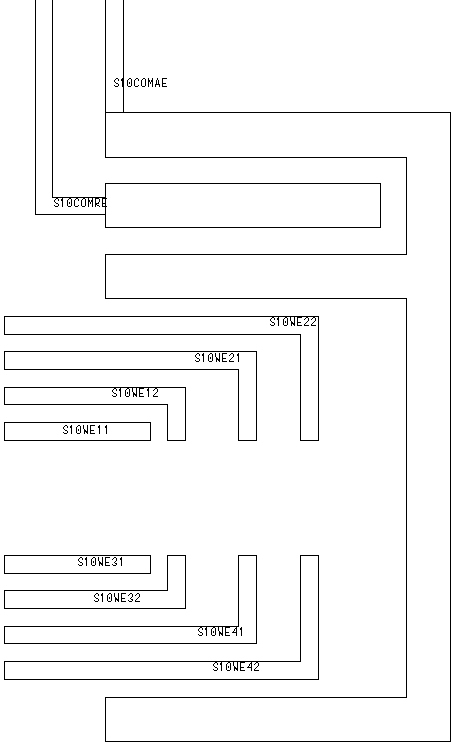
\includegraphics[height=\linewidth]{figures/s10.png}
\caption{Sensor 10 diagram.}
\label{sensor-10}
\end{figure}

The HDV shows the optimum potential for this electrode measuring NE is 0.85V (Fig. \ref{hdv}), which is near the typical value. There is an argument, however, to using a value less than 0.85V in order to decrease noise (other chemicals being reduced), which would also decrease the resulting signal. Since we are already near or perhaps at or limit of detection, though, the added noise is acceptable in order to maximize the output.

\begin{figure}
\centering
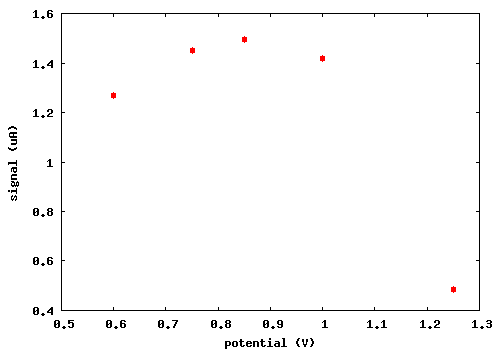
\includegraphics[width=\linewidth]{figures/hdv.png}
\caption{HDV; highest point at $0.85V$.}
\label{hdv}
\end{figure}

Concentration response characterization shows reasonable results in the 25$\mu$M to 200$\mu$M range (Fig. \ref{char}). For 2 pads, the expected output in amperes is $I = C * 2.22604*10^{-12} + 2.28364*10^{-11}$, where $C$ is the molarity of NE. For 4 pads, the expected output in amperes is $I = C * 4.16884*10^{-12} + 2.52294*10^{-11}$, where $C$ is the molarity of NE. As expected, the 4-pad set has a sensitivity slightly less than twice that of the 2-pad set. However, both best-fit lines do not, as expected, cross the origin, and thus suggest a constant amount of background current not dependent on senor area. It is not known---though it is suspected---whether a potentiostat with improved sensitivity (e.g., into the picoamp range) would be able to reliably detect concentrations below 25$\mu$M.

\begin{figure}
\centering
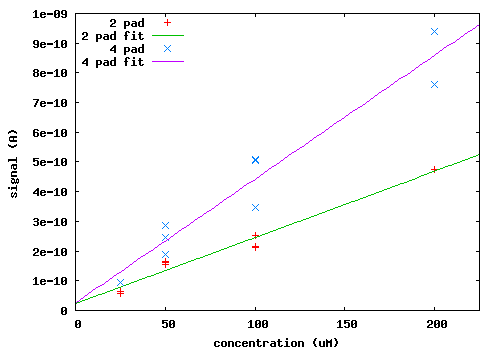
\includegraphics[width=\linewidth]{figures/char.png}
\caption{2- and 4-pad characterizations with 1st order best-fit lines.}
\label{char}
\end{figure}

Ovary test results show our potentiostat is not sensitive enough to detect possible NE releases from the cell. As we expect releases in the nanomolar and subnanomolar range, which we cannot currently detect due to potentiostat limitations, this is expected \cite{amperometry-review}. The three injections at the end of the testing are not statistically differentiable and do not correspond to our expectations of what should occur. It could also mean the chip sensors were damaged or restricted during ovary attachment and cannot function as expected.